\chapter{绪论}
\label{chap01}
近年来,随着互联网技术的发展,在线社交网络(Online Social Networks)在全世界范围内普及开来,其应用融入到了人们生活的方方面面之中。近十年来,对于在线社交网络的研究一直持续增长。在很大程度上,这归功于社交媒体以及社交服务网站的蓬勃发展。这些媒体以及网站的迅猛发展给社交网络分析(Social Network Analysis)提供了丰富的语料库与数据集。而对社交网络的研究与应用也促进了社交媒体以及社交服务网站的持续发展。在线社交网络是社会中个体集合以及个体之间连接关系所构成的网络在网络空间上的映射,即在线社交网络是真实社会在虚拟网络中的体现和拓展。在线社交网络拉近了人与人之间的距离,加快了信息传播的速率,丰富了群体的结构关系。因此,在线社交网络成为了社会学、传播学、计算机科学以及系统科学等领域的研究热点。

在线社交网络是在信息网络上由用户集合以及用户之间关系所构成的社会性结构,一般而言包含三个要素:“关系结构”、“网络群体”以及“网络信息”\upcite{方滨兴2014在线社交网络分析}。三个要素之间相互关联、相互依存,其关系如图\ref{fig:threeFactors}所示。其中关系结构为网络群体的互动行为提供了基础结构以及底层平台,是社交网络的载体;网络群体推动网络信息传播,影响关系结构的演化,是社交网络的主体;网络信息的内容和传播是社交网络关键点,是群体行为的诱因和效果,同时也影响关系结构的变化,是社交网络的客体。

\begin{figure}[!ht]
    \centering
    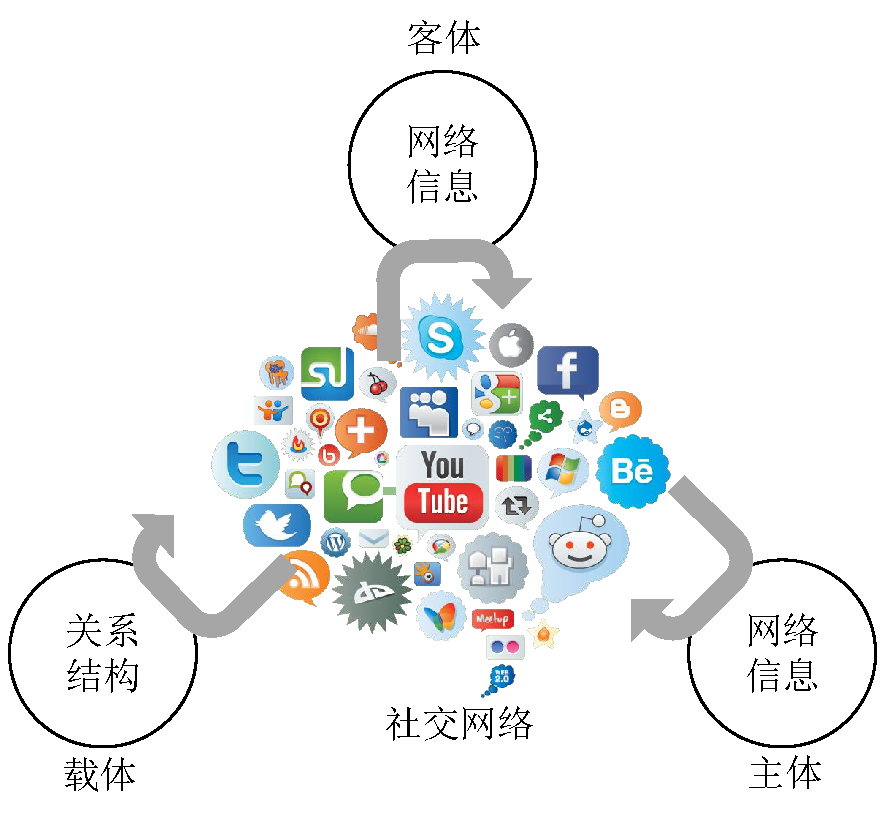
\includegraphics[width=0.5\textwidth]{threeFactors}
    \caption{在线社交网络中的关系结构、网络群体和网络信息}
    \label{fig:threeFactors}
\end{figure}

与传统的Web应用和信息媒体相比,在线社交网络具有如下的新特性:
\begin{itemize}
	\item 高速性:信息发布和接收十分便捷、迅速。社交网络中的用户可以通过手机、笔记本、电脑等终端,随时随地发布和接收信息,信息传递的效率高,具有高速性。
	\item 扩散性:裂变式的信息传播。社交网络中的信息一经发布,便会立刻推送给所有的关注者。信息经过转发,信息又将传播到下一批关注者。信息的传播呈现一种链式反应的几何级数扩散模式,为普通网民传播信息提供了渠道。
	\item 平等性:人人都有可能成为信息输出者。与传统信息媒体中信息发布和信息接收的非对称性相比,社交网络中的每一个参与者都有机会通过社交网络表达自己的观点,传播自己的信息,输出自身的价值观。因此,社交网络在热点事件的产生、发酵、传播等环节中扮演了重要的角色。
	\item 自发性:呈现自媒体形态、自发地形成虚拟社区。社交网络中的个体既是信息的接收者也是信息的发布者,用户会根据自身不同的关注内容与其他用户建立联系,形成网络中的虚拟社区。
\end{itemize}

这些丰富的特性让在线社交网络具有和其他信息媒体不一样的特点,同时也对信息安全提出了新的挑战。对于社交网络分析的研究,在结构、群体以及信息等方面都存在很多已有的工作。其中很多研究工作是关于网络中的信息传播、影响力、传播模型等。这些工作主要研究是否可以建立模型来解释信息的传播方式,如何在真实社交网络信息传播数据集上验证传播模型等等,这些仅仅是社交网络中信息传播研究的一些研究举例。信息传播在实际生活中有着许多应用,例如商业产品或者理念的推广营销、网络流量的爆发检测、寻找关键博客来获取重要的信息、寻找意见领袖或者潮流引领者以及信息的检索排序等等。

社交网络中信息传播关键技术的研究对于理解信息传播的机理有着重要的意义。本文首先在结构上进行理论研究,思考在社交网络中如何选取源节点才能使得信息传播效率更高,提出了传播效率最大化问题。然后,本文在内容方面进行分析,思考社交网络中不同用户的文本内容推送问题。本文利用语言模型以及深度学习等技术,对普通文本信息以及数据流信息进行应用,进行了基于语义扩展和文本质量的实时个性化搜索研究和基于卷积神经网络的文本分类研究,分析不同用户的关注点,将用户所感兴趣的、高质量的信息自动地推送给用户,使得用户更加便捷地获取信息,从而推动信息的传播。最后,本文在传播效果的评估方面进行分析,研究合理的传播模型。本文建立基于概率阅读的传播模型,对于事件的传播影响进行评估,来估测事件传播影响面的大小。本研究对于揭示信息传播的机理和规律、推动社交网络中的信息传播、发现有价值的信息以及保护信息安全起到了重要的作用。

本章首先对本文的研究背景进行阐述,第\ref{sec1:background}小节对在线社交网络中信息传播研究的发展现状进行描述,分析社交网络信息传播分析的研究意义和面临的挑战。其次,第\ref{sec1:relatedWorks}小节对本文研究的各个相关工作进行概述和总结。然后,第\ref{sec1:inovation}小节介绍本文的主要研究内容和创新点。最后,第\ref{sec1:paperStructure}小节给出了本文的组织结构。

\section{研究背景及意义}
\label{sec1:background}
本节主要介绍本文研究的背景及其意义,对涉及到的概念进行详细的阐述,对研究所面临的挑战进行分析。首先,本节对在线社交网络进行一个概述,介绍在线社交网络的起源、定义、特点以及发展状况。其次,本节对社交网络中的信息传播进行介绍,详细地描述信息传播的特点及其所涉及到的因素。然后,本节对本文的研究的意义进行总结。最后,本节分析了研究所面临的挑战。
\subsection{在线社交网络概述}
\label{subsec1:introduction}
人类自诞生以来,就过着群居的生活,一同劳作、交流以及分享,从而形成了社会。随着人类文明的发展和社会的进步,人与人之间的关系进一步的深入和加强,社会关系由简单的血缘关系向朋友关系、雇佣关系以及社交关系发展。而人与人之间由生活、工作、学习、娱乐等等社会交互而形成了某种稳定的关系,这一系列的关系将社会个体结合成了一个巨大的网络,这即是社交网络。如同Linton Freeman所说的那样,我们都被一个无形的网络连接在一起\upcite{freeman2004development}。

社交网络(Social Network)在维基百科中被定义为由社会个体(例如个人或者机构等)、社会个体间的二元关系以及社会个体之间的社交互动组成的社会结构\upcite{social_network}。在社交网络中,个体之间因为社交互动而形成相对稳定的关系体系,这种关系可能是亲属关系、朋友关系、同学关系,也可能是商业合作关系或者宗教信仰关系等。通过这些关系,社交网络把偶然相识的弱关系到紧密结合的强关系,以及社会中各式各样的人群串联成了一张巨大的网络。由于社交网络中存在各种各样的社会关系,个体之间的网络结构往往是非常复杂的。而且,复杂的关系结构也会影响网络中个体之间的社交互动,进而影响到个体的社会行为。

随着工业化、城市化的进行以及移动网络的发展,社会网络化的趋势日益凸显。在2012年,Lee Rainie和Barry Wellman在其著作《网络化:新的社会操作系统》\upcite{rainie2012networked}中指出,社会网络革命、移动革命以及互联网革命将是影响人类社会发展的三大革命。随着互联网的进步,网络结构受地域性因素的影响减弱了,这使得跨地域性的线上社会关系成为了社交网络的主要形式。在现实社会中,人们相继在社交媒体平台上创建账号,将线下的社会关系扩展到了线上,并且进一步的延伸,这使得在线社交网络成为了人们网络生活中不可或缺的沟通工具。

在2009年欧盟关于社会计算的研究报告中\upcite{huijboom2009key},在线社交网络主要可以分成如下的四个大类,
\begin{itemize}
	\item 即时通讯应用。这一类的应用提供一个实时的通信平台,使得人与人之间能够通过网络进行在线的交流、信息的分享等。典型的代表有MSN、QQ、飞信等,其具有双向认证与实时推送的特点。
	\item 在线社交应用。这一类的应用提供一个在线社交关系平台,人们在平台上进行社交互动以及消息的共享等。典型的代表有脸书(Facebook)、谷歌+(Google+)、人人网、QQ空间等,其具有双向认证以及非实时推送的特点。
	\item 微博类型应用。这一类的应用提供一个自媒体的信息发布平台,任何个人或者机构都能在平台上发布信息,推送给其关注者。典型的代表有推特(Twitter)、新浪微博、腾讯微博等,其具有单向认证以及实时推送的特点。
	\item 共享空间以及其他应用。这一类的应用提供一个公告发布系统,具有沟通功能,但是用户之间结合不紧密。典型的代表有BBS、论坛、博客等,其具有单向认证以及非实时推送的特点。
\end{itemize}

社交网络是Web 2.0时代的具有代表性的应用,具备Web 2.0时代交互性、主动性的特点,众多社交软件应用随着技术的更新而蓬勃发展。中国流行的即时通信软件“腾讯QQ”诞生于1999年,在2016年的月活跃账户数(MAU)达到8.77亿,其中智能终端月活跃账户达到6.47亿\upcite{tencentReport2016}。2004年于美国上线的社交网络服务网站脸书(Facebook)成为了全球范围内最流行的社交网站之一。从网站成立至今,其用户持续增长,在2016年第四季度,脸书月活跃人数已经突破了18.6亿,其中移动端用户数达到了17.4亿\upcite{facebookReport2016}。2006年微博客类的应用推特(Twitter)在美国诞生,允许用户更新不超过140个字符的消息,成为一个广受欢迎的社交网络及微博客服务网站。截至2016年第四季度,推特的平均月活跃用户为3.19亿\upcite{twitterReport2016}。随着全球社交网络的发展,相似的网站在国内也纷纷出现。2009年,新浪微博正式上线,政府、明星以及草根用户等社会各界人士纷纷开设账户,发布和接收信息。截至2016年底,新浪微博的月活跃用户数达到了2.97亿,其中89\%的用户为移动端用户,平均日活跃用户(DAU)达到了1.32亿\upcite{weiboReport2016}。腾讯在2011年推出的一个为智能终端提供即时通讯服务的软件“微信”在当今已经成为了新时代移动端即时通讯的领军,微信和WeChat(微信的海外版)在2016年的合并月活跃账户数达到8.46亿\upcite{tencentReport2016}。

随着网络科技和设备产品的飞速发展,社交网络逐渐成为人们接收传播信息、发表自身观点以及讨论公共事件的主要渠道。根据中国互联网络信息中心(CNNIC)发布的第39次《中国互联网络发展状况统计报告》显示,截至2016年底,中国网民的规模达到了7.31亿,与欧洲的人口总量相当,互联网的普及率达到了53.2\%。其中手机网民占比达到了75.1\%,规模达到6.95亿,增长率连续三年超过10\%,移动互联网极大地丰富了网民获取信息的通道\upcite{cnnic2017zghlwfzbg}。随着网民数量的增长,社交网络中的信息量也随之上升。推特中每天产生的信息突破了0.58亿条,查询次数突破了21亿次\upcite{statisticbrain2017twitter}。脸书平均每20分钟就有1百万条链接被分享、3百万条信息发布\upcite{statisticbrain2017facebook}。2017年的春晚直播期间,在新浪微博平台中讨论春晚的微博数量达到了近6千万条,网友互动量达1.99亿次,共有超过1.2亿网友参与到了微博抢红包的活动中\upcite{techsina2017newyear}。2017年的除夕,国人在微信和QQ平台上使用红包互送祝福,其移动支付峰值达到了20.8万笔/秒,合计支付总数达到了32.2亿笔\upcite{techqq2017luckymoney}。由以上数据可以看出,社交网络为人们生活的各方面都提供了平台,成为了人们获取、发布以及传播信息的关键渠道。

% 社交网络之所以能够如此迅速的流行起来,是因为它具有如下一些特点。首先是社交网络简单易用。任何个人或者组织都能够随时随地发表言论,分享内容。而且,用户接收和发布信息的渠道多种多样,可以在互联网的客户端,也可以在移动客户端。这些都极大地加速用户接收、发布和传播信息的速率,使得信息在群体之间的传播更加的高频化。其次是社交网络交互频繁。社会个体通过关注/被关注、好友等关系紧密联系在一起,网络结构复杂。群体之间通过兴趣爱好、共同关注点等因素形成较为固定的社区,社区内部的成员在同一个话题上相互讨论、分享。与传统信息媒体不同,社交网络中的社会个体既是信息的接收者,又是信息的传播者,同时还可能是信息的传播者。这些因素都促进了社交网络中信息的产生与传播。然后是社交网络与现实社会相互映射。随着社交网络的发展,越来越多的个人和机构在社交网络中实名认证,在网络世界中与人们交互来提高自身的影响力。这进一步地拉近了虚拟和现实之间的差距,真实社会中发生的事件将会迅速的在社交网络中以信息的形式发布与传播。

% 由于上述的原因,社交网络迅速崛起,在短时间内吸引了大量的用户加入。用户在社交网络中分享现实社会中发生的事件,发表自己的意见,这也使得虚拟网络和现实世界的界线逐渐模糊。由于网络资源的公开性以及透明性,社交网络中的数据相对于现实世界要易于获取,这使得一些原本在现实世界中难以研究的内容存在了研究的可行性。研究者可以分析虚拟网络中的数据,并通过现实世界在虚拟网络中的映射,间接来研究现实世界中的问题。例如人口年龄分布问题、政策满意度问题、舆论热点分析等等都可以在社交网络中得到较好的解决。正因如此,社交网络的出现促进了社会学、传播学、系统科学、计算机科学等学科新一轮的发展。

\subsection{社交网络信息传播}
\label{subsec1:informationDiffusion}
在线社交网络与生俱来的自由性和开放性,使其成为了现代社会中信息传播的重要渠道,社交网络中的信息传播活跃度达到了前所未有的程度。信息传播(Information Diffusion)是指个体、组织之间的信息传递和交流\upcite{baike2017info}。人们通过符号、信号等信息载体来接收、传递与反馈信息的活动,人们相互交换思想和意见等,以达到相互影响和了解的过程。而社交网络信息传播指的是以社交网络为媒介进行信息传播的过程\upcite{方滨兴2014在线社交网络分析}。1948年,Lasswell在《社会传播的结构与功能》\upcite{lasswell1948structure}一文中指出了传播过程及其“5W”要素,即:谁(Who),说了什么(Says What),通过何种渠道(In Which Channel),对谁(To Whom),造成了什么结果(With What Effect)。经典的5W传播模式构成了传播学中研究的五个基本内容,即控制研究、内容分析、媒介研究、受众研究以及效果研究。

社交网络信息传播影响着生活的各方各面,并且改变人们的行为模式。2007年,Christakis和Fowler在新英格兰医学杂志上的发表文章\upcite{christakis2007spread},研究分析了12,000名患者的药物记录,并根据患者之间的亲属关系、邻居关系等,从药物记录中抽取了一个离线的社交网络。研究的目的是分析非传染病(例如肥胖症等)与患者社交网络邻居的关系,理解具有患非传染病网络邻居和自身患有该非传染病的关联关系。在不考虑其他原因的情况下,研究表明拥有肥胖症患者朋友会使得自身也患肥胖症的风险提高171\%。这说明了肥胖症患者会通过社交网络把容易导致肥胖的习惯传播给其网络邻居。该研究主要把重点放在了关联关系上,而不是患病原因,研究结果表明了社交网络间传播影响的效应。在Christakis和Fowler的另一个研究中,吸烟这一个行为也在社交网络中的传播影响也得到了印证\upcite{christakis2008collective}。在2011年,Christakis和Fowler在其著作\upcite{christakis2009connected}中指出了传播的重大影响,并解释了社交网络的组成和运作机理。其中包含了很多真实的案例,例如背痛的症状自柏林墙推倒后从西德传入东德,自杀倾向通过社团传播,政治倾向和信仰通过网络传播等。而在商业圈,信息传播引领成功的最为著名的案例是“Hotmail现象”\upcite{hugo2001emergence}。在20世纪90年代初,Hotmail是一个相对冷门的邮件服务提供商。为了改变这个局面,公司使用了一个相对简单的创意,即在每一封用户发送的邮件结尾自动地加上“欢迎加入世界上最大的邮件服务提供商MSN Hotmail”这一宣传语。这一宣传语通过用户之间的邮件传播,加速了品牌的树立和传播。在短短18个月后,Hotmail就成了世界第一大邮件服务提供商,拥有了800万用户。在2012年7月发布的一首韩国流行歌曲“江南style”成为了YouTube上最先突破10亿观看的节目。而在另一方面,社交网络中的信息传播在社会的突发事件中也有着体现。在2011年夏天,加拿大温哥华举办的史丹利杯冰球决赛引发了骚乱。其中许多是青少年,他们破坏了城镇中的财物,并且在社交媒体上自吹自擂,例如发布图片、视频等。这引发了广泛的传播,并且成为了法庭的取证。相比于现场的证据,社交媒体中的证据种类更多。这使得警方在短时间内确认了骚乱者的身份。

社交网络中的信息传播具有以下特点。首先,社交网络中的信息发布与接收十分便捷、快速,用户可以通过手机等移动设备随时随地发布和接收信息。其次,社交网络中的信息传播的扩散形式呈“裂变式”扩散。消息一经发布将即刻推送到关注者,而关注者的转发将产生下一轮的传播。然后,社交网络中的每一个用户都有成为意见领袖,热点制造者的可能,所有网民都可能在热门事件的传播中扮演重要的角色。最后,社交网络中的信息传播呈现“自媒体性”,任何一个用户或者机构都能够建立属于自己的媒体,通过发布信息、制造热点、传播信息来扩大自身的影响力。这些特点使得社交网络中的信息传播更加迅捷、传播范围更广,人们在社交网络中的交互更加的频繁。

社交网络信息传播之所以有如上的特点是由于如下几个因素\upcite{方滨兴2014在线社交网络分析}。首先是关系结构。社交网络中的个体基于相互认识、兴趣爱好或是个人崇拜等原因,在社交网络上形成了复杂的关系结构。其次是网络群体。基于社交网络中的关系结构,网络个体因为关系而大量聚合,并且相互作用、相互影响,从而形成具有不同特征的网络群体。最后是网络信息。社交网络中的关系结构提供了底层的高速传播通道,网络群体直接助力网络信息的传播,丰富的网络内容提供了信息资源。关系结构、网络群体以及网络信息的有机结合加速了网络信息的传播。

\begin{itemize}
	\item 网络结构。社交网络中的个体间进行丰富的交互,形成了“一对一”、“一对多”、“多对多”以及“多对一”几种传播模式的组合。网络结构中节点间的连接强度和网络密度各不相同,从而形成了不同的连接关系。强连接会导致形成紧密联系、聚集的社区结构,意见更加统一;弱连接通常在关系不紧密、联系不频繁的个体间形成,可以提供新的信息,丰富了信息的内容,扩大了传播范围。
	\item 网络群体。网络个体聚合并且相互影响、形成了网络群体。与现实世界中的群体相比、网络群体传播具有高度的互动性、开放性、跨地域性等特点。网络群体中的意见领袖往往具有较大的影响力,能够引领其所在群体对于事件的倾向性和态度。
	\item 网络信息。网络信息具有时效性、多源性、多样性等特点,在信息传播时起着不可或缺的作用。社交网络的信息的源头不仅仅是网络中的链接信息,而且来自于传统媒体的信息接入。网络信息在社交网络中传播会产生相互影响,与独立信息的传播不同,可能引发更多的讨论和演化。
\end{itemize}

社交网络信息传播由于这些新的因素的出现,凸显出与传统信息传播的不同特性,加速了信息传播的效率和多样化。在实际生活中影响到人们的各方各面,在给人们带来巨大便利的同时,也对信息安全提出了新的挑战。
\subsection{研究意义}
\label{subsec1:researchSignificance}
研究社交网络中信息传播对科学研究、社会安全以及商业发展都是十分有意义的。研究社交网络中的信息传播规律,有助于加深我们对于社交媒体的理解,解释社会中发生的现象,同时使得我们对于复杂的网络拓扑结构、传播能力以及网络动力学等有着进一步的认识。

从科学研究的角度来讲,研究社交网络中的信息传播更有益于理解信息的传播机理,方便推动或者干预信息在人类社会的传播。随着社交网络的发展,各类社交媒体的兴起,用户在网络上发布信息的数量呈爆炸式增长,这些信息通过社交网络这一个良好的渠道在用户之间迅速传播。社会中的事件都会在网络中得到体现,用户将分享个人的生活、讨论热点事件、发表政治观点等等。社交媒体中的信息量已经逐渐超越了传统的新闻、博客等应用的信息量,社交网络成为了信息传播的主要平台。信息在传统的媒体中传播往往通过线上线下的口口相传等途径,而这些方式难以形成记录。社交网络中的信息传播有迹可循,能够记录其传播轨迹,这为开展相关研究提供了丰富的数据基础,使得研究人员有机会在海量的真实数据上建立模型,研究信息传播机制,认识传播规律。

从社会安全的角度来讲,研究社交网络中的信息传播能够使得人们及时接收到真实的信息,免受谣言的危害,保护社会公众的安全与财产。社交网络融入了人们的日常生活,改变了人们的生活方式,影响到包括政治、教育、经济、文化等等方面。在政治方面,微博已经直接在很多政务活动中发挥了巨大的作用。在2008年的美国大选中,奥巴马及其团队利用社交媒体推特进行了助选活动,在推特上制造舆论,争取选票。奥巴马接受竞选总统提名的演讲创下了推特每分钟发表推文5.2万条的记录。在当选之后,奥巴马及其团队继续利用社交网络提高政治影响力。在教育方面,美国的众多大学纷纷在社交网络上发布公开课,直接支持远程教育,并且在脸书和推特上与慕课(MOOC)进行资源整合。在经济方面,电子商务已经成了人们的主流购物方式之一。众多的公司通过社交网络进行宣传,提升自身品牌的竞争力,最终提高了营业额。在文化方面,社交网络正在改变人们的生活方式,足不出户便能与世界各地的网友进行互动,直播平台、虚拟现实技术的诞生使得人们的交互体验更加的多样化。与此同时,社交网络中的信息传播也会给社会带来负面影响。在政治方面,不法分子蓄意制造和传播有害国家安全和社会利益的谣言,影响社会稳定。我们民众曾多次受到微博谣言的影响而发生“抢盐”风波。在教育方面,邪恶势力通过社交网络蛊惑青少年崇尚暴力,灌输错误思想,怂恿其破坏社会的稳定。在经济方面,网络诈骗者利用社交网络发布虚假信息,进行诈骗活动,损害人们的经济利益。在文化方面,犯罪团伙利用社交网络,传播网络色情以及暴力信息,而且往往伴随着传播网络病毒、木马等行为。

在商业发展的角度来讲,研究社交网络中的信息传播能够使得个人、公司或者组织抓住机遇和挑战,实现自身利益的最大化。个人通过社交媒体发布自己的观点、看法,成为社交网络中的意见领袖,形成自媒体。社交网络使得推广自己更加的便捷、简单。例如,罗振宇在社交网络中推广“罗辑思维”节目而走红,成为了自媒体“首富”。而互联网企业通过分析社交网络中的趋势,制定自身的战略方向,通过社交网络发布自己的产品或者理念,能够快速地推广自身的产品。同时,社交网络中的个人信息透明化,使得个人隐私更容易被利用,这对隐私保护提出了新的要求。社交网络中信息传播速率快,传播范围广,这对企业的公关能力提出了挑战。

综上所述,社交网络的发展对社会各方各面都带来了机遇和挑战,同时也对人们提出了新的要求。研究社交网络信息传播有助于理解传播的机理,提高应对突发事件的能力,促进经济的繁荣发展,对于政治经济安全、国家社会稳定以及企业个人财产利益都有着重要的意义。
\subsection{面临的挑战}
\label{subsec1:challenge}
在线社交网络中信息传播分析与自然语言处理、数据挖掘、机器学习、海量数据处理、传播学、社会学等等学科有着紧密的联系。社交网络带来了丰富的语料数据和结构关系,但是也提出了新的挑战。尽管与之相关的各个领域的研究已经取得了很多的成果,提供了相应的技术支持。但是,由于在线社交网络中的信息传播同以往的研究存在诸多不同之处,这一研究依然面临着新的问题与挑战,具体包括如下几个方面。

\begin{itemize}
	\item 数据的海量性。社交网络信息传播分析所涉及到的数据量往往是海量的,这对信息传播的分析提出了较大的挑战。数据的海量性体现在两个方面,一个是信息内容海量,二是用户结构海量。这对信息传播的分析算法处理数据的能力提出了新的要求。在一些热点突发事件的爆发过程中,社交网络中的信息往往在短时间内便会达到一个较大的数量级,例如2016年奥运会中的中国女排夺冠,“女排精神”成为了国人共同的关注点,女排夺冠相关内容互动量在当天达到了7285万次,相关视频播放量达到3.4亿次\upcite{sina2016volleyball}。信息传播分析通常需要分析文本的内容,分析用户之间的传播关系等,如何实时地处理如此庞大的数据是社交网络信息传播需要研究的问题。
	\item 文本的多样性。社交网络中的文本形式多样,微博类的应用通常限定用户的文本长度不超过140个字符。而新闻、论坛或者微博中的长博文则对用户发表文本的长度没有严格的限制。这使得传统的文本表示模型在社交网络中,对长短文本的处理性能明显下降,在文本分类、文本聚类、信息推荐等应用方面影响较大。因此,社交网络中的信息该如何表示对社交网络中信息检索、信息推荐等应用提出了新的挑战。
	\item 结构的复杂性。社交网络中的用户数量庞大,而且不同社交媒体之间的用户存在着重叠现象。社交网络中的用户通过朋友、兴趣等多种关系聚合在一起,形成多种多样的复杂结构。计算信息传播的影响范围、信息的溯源以及如何选择节点使得影响力最大化这些问题在社交网络环境中都出现了新的挑战,传统的方法的性能在复杂的网络中效率明显下降。如何在复杂的网络中快速地、有效地对信息传播进行分析对抽样理论、算法设计等都提出了挑战。
\end{itemize}

由此可见,社交网络的发展对信息传播研究提出了多方面的挑战,同时,也为信息传播研究提供了丰富的数据和渠道,这也为信息传播的研究提供了一个虚拟的环境。

\section{相关研究工作}
\label{sec1:relatedWorks}
社交网络中的信息传播相关的工作涉及到的研究十分广泛,包括自然语言处理、数据挖掘以及机器学习的各种研究方法。本小节主要从传播源的选择、信息内容的选择以及传播效果的评估等方面介绍相关的研究工作。其中涉及到的相关工作有影响力最大化、实时个性搜索、语言模型与文本分类以及传播模型的学习等相关研究。
\subsection{影响力最大化}
\label{subsec1:influenceMax}
影响力最大化问题的实际应用是通过信息传播来推广新产品、新理念以及新政策等。为了实现网络中信息的迅速传播,主要有研究分为两个方向。第一个方向是传播模型的建模,第二个方向是寻找一个快速有效的方法来找到具有影响力的个体。

对于第一个方向,已有很多工作对传播模型进行了深入的研究。均匀模型(Uniform Model)假设所有节点的影响概率为一个常数(例如0.01),该模型不区分节点之间的关系。首先,每一个节点都以相同的概率影响其邻居节点,模型未能区分节点对于其他节点的影响力。其次,每一个节点受到其邻居节点的概率也是相同的,模型未能区分不同邻居节点对该节点的影响力。显然,这样的假设是值得商榷的。三态模型( Trivalency Model)在一定程度上解决了第一个问题,节点的影响概率为一个集合中的某一个元素,例如$\left\{ 0.001, 0.01, 0.1\right\}$。模型的思想是对不同影响力的节点赋予不同的影响概率值。上述的两个模型的影响概率与网络的结构无关。在加权级联模型(Weighted Cascade Model)中,模型定义影响概率与网络的边$\left(u,v\right)$相关,影响概率$p_{uv}=1/d_{in}v$,其中$d_{in}v$为节点$v$的入度。该模型比均匀模型和三态模型拥有更好的性质。首先,低入度的节点受到其入度邻居节点的影响要大于高入度的节点。这样影响概率不仅仅是从一组常数中进行选择。其次,一个节点对于出度节点的影响不再是相同的,这是由于这些出度节点的入度不同。然而,加权级联模型仍然无法解释节点之间的影响概率是如何计算得出的。Saito等人\upcite{saito2008prediction}研究了如何学习影响概率的问题,主要以独立几联模型为研究对象。通过观测信息传播过程中的每个时间段,来求解设定影响概率为参数下的极大似然估计,从而求解影响概率。在线性阈值模型中,每个节点存在一个阈值$\theta \in \left[ 0,1 \right]$,当累计影响超过阈值时,节点将被激活。Goyal等人\upcite{goyal2010learning}通过社交网络中的信息传播轨迹来学习节点之间的影响概率。

对于第二个方向,影响力最大化问题最早是由Domingos和Richardson所提出,问题基于马尔科夫随机场(Markov Random Field)进行建模\upcite{domingos2001mining,richardson2002mining}。随后,Kempe等人将影响力最大化问题建模成一个离散的随机优化问题\upcite{kempe2003maximizing}。影响力最大化的问题可以定义为如下所示,

\begin{defn}[影响力最大化问题]
\label{def:imProblem}
影响力最大化问题可以形式化为如下一个随机优化问题:给定一个图$\mathcal{G} = \left(\mathcal{V}, \mathcal{E}\right)$、图$\mathcal{G}$上的一个随机传播模型以及一个阈值$k$。给定一个种子节点集合$S \subseteq \mathcal{V}$且满足$\left\vert{S}\right\vert \leq k$,则集合$S$的影响力期望为$\mathbb{E}_\mathcal{G}\left[I\left(S\right)\right]$。则影响力最大化问题为寻找使得影响力期望最大的集合$S^{\ast}$。问题可表示为如下所示,
\begin{equation}
\label{eq:imProblem}
    \begin{split}
        &S^{\ast} = \arg\max{\mathbb{E}_\mathcal{G}\left[I\left(S\right)\right]}\\
        &s.t.~~S \subseteq \mathcal{V},\left\vert{S}\right\vert \leq k
    \end{split}
\end{equation}
\end{defn}

在给定了一个传播模型后,例如独立级联模型(Independent Cascade Model)或者线性阈值模型(Linear Threshold Model),影响力最大化问题可以分解成两个问题。第一个问题称为影响力期望计算问题,即给定了一个种子节点集合$S$后计算其影响力期望$\mathbb{E}_\mathcal{G}\left[I\left(S\right)\right]$。第二个问题是如同定义\ref{def:imProblem}所示,找到使得影响力期望最大的种子节点集合。

对于影响力期望计算问题,Wang等人\upcite{wang2012scalable}以及Chen等人\upcite{chen2010scalableLT}证明了其复杂度在独立级联模型和线性阈值模型下是\#P-难的。\#P问题是计数问题,与NP问题中决策问题相关。NP问题需要求解一个问题实例是否存在解,例如合取范式(Conjunctive Normal Form)方程是否存在可满足解,而\#P问题需要求解这个问题实例存在多少个解,例如合取范式方程存在多少个可满足解。如果一个问题是\#P的且每一个\#P的问题都可以在多项式时间内归约到它,那么这个问题是\#P-完全的。如果一个问题可以在多项式时间内由一个\#P-完全的问题归约到它,那么它是一个\#P-难的问题。对于独立级联模型或者线性阈值模型,上述的证明过程都可以由一个\#P-完全的问题,$s$-$t$连通性问题\upcite{valiant1979complexity},来进行归约。

对于寻找影响力期望最大的种子节点集合的问题,Kempe等人\upcite{kempe2003maximizing}给出了结论,问题的复杂性在独立级联模型和线性阈值模型下都是NP-难的。其证明思路将NP-完全的问题归约到影响力最大化问题。在独立级联模型中,证明将子集覆盖(Set Cover)问题归约到影响力最大化问题;而在线性阈值模型中,证明将节点覆盖(Vertex Cover)问题归约到影响力最大化问题。

上述研究表明了影响力最大化问题是一个复杂性较高的问题。问题的难度来自于两方面,一方面是问题的组合性质,另一方面是计算影响力期望的难度(甚至是计算一个节点的影响力期望)。针对这两个问题,已有的研究主要应用贪心算法来解决组合问题,利用蒙特卡罗(Monte Carlo)模拟来解决影响力期望计算问题。对于影响力最大化问题使用贪心算法能够得到一个下界的保证,即运用贪心算法得到的解最差的结果有理论性的保证。这是由于影响力期望函数$\mathbb{E}_\mathcal{G}\left[I\left(\cdot\right)\right]$具有两个很重要的性质,即子模性(submodularity)和单调性(monotonicity)。子模性的定义如下所示,
\begin{defn}[子模性]
\label{def:submodularity}
子模性的定义可以解释为往种子节点集合加入更多节点时,所造成的效果为边际收益递减(Diminishing Marginal Returns)。对于一个集合函数$f:2^{\mathcal{V}} \rightarrow \mathbb{R}$,如果对于任意的子集$S \subseteq W \subseteq \mathcal{V}$且任意的元素$v \in \mathcal{V} \setminus W$,将元素$v$加入到集合$W$中的边际收益不超过将元素$v$加入到集合$S$中的边际收益,那么函数$f\left( \cdot \right)$具有子模性,用公式表示如下,
\begin{equation}
\label{eq:submodularity}
	f\left(S\cup\left\{v\right\}\right) - f\left(S\right) \geq f\left(W\cup\left\{v\right\}\right) - f\left(W\right)
\end{equation}
\end{defn}

另一个重要的性质单调性定义如下,
\begin{defn}[单调性]
\label{def:monotonicity}
单调性的定义可以解释为往集合中增加元素不会使得函数值变小。一个集合函数$f:2^{\mathcal{V}} \rightarrow \mathbb{R}$,如果对于任意的子集$S \subseteq W \subseteq \mathcal{V}$,都有$f\left(S\right) \leq f\left(W\right)$,则函数$f\left( \cdot \right)$具有单调性。
\end{defn}

对于具有子模性和单调性的函数$f\left( \cdot \right)$,Nemhauser等人\upcite{nemhauser1978analysis}证明了使用贪心算法得到的解的性能存在着下界。令$S^{\ast}$表示问题的最优解,函数$f\left( \cdot \right)$具有子模性和单调性且满足$f\left( \emptyset \right) = 0$,$S^g$为通过贪心算法得出的解,则可以用公式表示为如下所示,
\begin{equation}
\label{eq:lowerBound}
	f\left( S^g \right) \geq \left( 1 - 1/\mathsf{e} \right) f\left( S^{\ast} \right)
\end{equation}
其中$\mathsf{e}$为自然对数的底。其证明过程\upcite{chen2013information}利用了单调性和子模性以及递推方法得到公式(\ref{eq:lowerBound})的结论。

对于影响力最大化的求解,Kempe等人\upcite{kempe2003maximizing}的研究是最早将影响力最大化问题当做优化问题来求解的,并且给出了贪心算法的求解。Leskovec等人\upcite{leskovec2007cost}提出了一种改进算法,CELF算法。算法利用函数的子模性来对于不必要的模拟进行剪枝,使用一个优先队列实现,在不改变输出的情况下提高了算法的性能。Goyal等人\upcite{goyal2011celf++}基于上述的工作进行了改进,提出了CELF++算法。Cheng等人为了解决可扩展性和准确度之间的矛盾,提出了一个静态的贪心算法,为StaticGreedy算法。该算法保证了信息传播过程中影响函数的子模性,在准确度不损失的情况下,极大地降低了运算量。Borgs等人提出了一种不同于贪心算法的新型框架,利用了反向传播抽样方法,极大地加速了算法的效率,同时保证了算法的性能。

基于影响力最大化问题,许多研究提出了基于此之上的衍生问题。传统的影响力最大化问题是种子节点集合的大小进行限制,阈值为$k$。Leskovec等人\upcite{leskovec2007cost}假设选择每一个节点都会产生开销,每一个节点的开销不尽相同,而总开销的大小固定作为限制,问题是在不超过总的预算下来产生最大的影响。在某些情况下,网络可能是动态的网络,在动态网络中研究影响力最大化问题\upcite{chen2015influential,zhuang2013influence}也是一个十分有意义的方向。Yang等人\upcite{yang2016continuous}对动态的影响力最大化问题进行研究,提出了一种通用的坐标下降算法来解决该问题。Wang等人\upcite{wang2015maximizing}在原问题的基础上,考虑了激活的节点以及最终传播到单未激活的节点(称之为已通知的节点)两类节点,提出了信息覆盖最大化问题(Information Coverage Maximization),并对该问题进行了求解。Liu等人\upcite{liu2012time}将传播时间纳入了考虑,提出了一种时间约束的影响力最大化问题。Shishir等人\upcite{bharathi2007competitive}考虑到了信息传播中多个传播源博弈游戏,对多源情况下的信息竞争传播问题进行了分析,对先手情况给出了求解方法。

\subsection{实时个性化搜索}
\label{subsec1:realTimeSearch}
实时个性化搜索的目的是根据用户偏好迅速地识别出用户所感兴趣的物品或者内容,涉及到许多的研究领域,包括个性化搜索、语言模型以及协同过滤等等。

在个性化搜索方面,根据不同的用户,对于检索内容进行重新排序是提高性能的一个常用的方法。Xie等人\upcite{xie2016personalized}针对上下文关系中的语言知识,使用图结构对语言知识的内容和相互关系建模,从而获取用户的偏好。同时,该工作提出了一个发现支配集的算法,来降低非相关上下文的影响,并提出了一个重排算法来衡量一次查询与信息的相关性、发现的文本内容与用户信息的相关性。Sontag等人\upcite{sontag2012probabilistic}针对特定用户的个性化搜索提出了一个新的方法。工作提出了一个关联生成模型,可以用来针对一次查询计算文本和用户的关联。生成模型中的用户相关的参数构成了一个用户的信息,可以通过用户长期的搜索记录来进行学习。Wang等人\upcite{wang2013personalized}针对搜索引擎对用户不区分的问题,提出了一种通用排序模型的适应性框架来解决个性化搜索问题。模型使用一个离线训练的用户无关的排序模型以及有限数量的不同用户的查询,能够更好的适应不同用户的搜索偏好。Tang等人\upcite{tang2015personalized}将个性化推荐问题形式化为一个上下文歹徒问题(\textit{contextual bandit problem}),来解决获取新的知识和基于已有知识做决策的相互制约问题。工作提出了一种非参数的策略,使用了一个有规则的重采样方法来得到需要估测模型的分布。根据概率匹配的模式,算法随机地从得到的分布中选取一个模型。Leginus等人\upcite{leginus2016personalized}针对推特中信息量繁多,而用户无法处理大量信息的问题,提出了个性词语云生成的方法来作为用户导航。用户的行为历史,例如发布的推文、转推、浏览的推文,都可用来提升词语云的个性化。Du等人\upcite{du2016folksonomy}对协同标签系统中个性化搜索中的用户建模进行了研究,通过标签以及排序等信息,提出了一种多层次的用户模型,实现个性化搜索。模型不仅能够反应出用户的偏好,也能反应出用户不喜欢的内容。Younus等人\upcite{younus2014language}针对个性化搜索引擎中的用户模型进行了研究,利用推特作为个性化搜索引擎的用户信息源,提出了一种统计语言模型,将推特中的用户特征考虑在内。个人化的用户模型使得检索的准确率得到了显著的提高。Xie等人\upcite{xie2014mining}针对社交网络中隐藏用户社区发现问题进行了研究,提出了增强分类图(Augmented Folksonomy Graph)的机制来包含社交网络中的多方面关系,同时基于一种新型的密度估计的聚类方法来寻找隐藏的用户社区。Li等人\upcite{li2015real}针对社交网络中的频繁信息更新以及小世界特性,提出了一种通用框架来解决个性化top-k查询问题。框架基于通用的排序框架,集成了时间新鲜度、社交相关性以及文本相似度特征。算法应用了一个三维立方倒排索引来支持在三个特征维度上有效的剪枝。然后提出了一个基于该立方的算法来检索top-k的结果。

在短文本的研究方面,由于社交网络中的文本具有不同的性质,包含了更多的标签以及结构化和非结构化的属性,因此对这方面的研究是十分有必要的。在社交网络中的信息检索方面,Massoudi等人\upcite{massoudi2011incorporating}为了解决社交网络中短文本信息量不足的问题,提出了一种检索模型,对特定话题检索微博中的博文信息。由于传统的信息检索模型在微博中无法直接适用,研究针对微博的特性设计了一种语言模型。算法通过文本特性和微博特性两方面对模型的性能进行提升,同时使用了一个动态的查询扩展模型来对微博博文检索进行处理。Severyn等人\upcite{severyn2015learning}使用了卷积神经网络来重排短文本对(查询-文档对),其中神经网络可以用来表示短文本对以及计算他们之间的相似度。该算法将词语当做输入,简化了预处理过程。该方法在TREC的两个常见的任务(智能问答以及微博检索)中显示了较好的性能。Ren等人\upcite{ren2014hierarchical}在社交网络流数据中的层次多标签的分类中进行了研究,由于概念漂移、种类之间的复杂关系以及社交网络数据流中的文本长度有限对该问题都提出了挑战。研究的核心思想包括短文本的扩展、时间感知的话题追踪和基于块结构的学习。Paik\upcite{paik2013novel}对信息检索中的词语权重问题进行了研究,提出了一种新型的tf-idf词语权重方法。算法使用了两种不同的文档词频归一化来得到两方面的词语特性。一种词频在短文本中效果较好,另一种在长文本中效果较好,最终的词语权重综合考虑了这两部分的影响。

在协同过滤搜索方面,由于社交网络中的信息和用户紧密相连,优质的用户更可能产生有意义的信息。Xue等人\upcite{xue2009user}针对传统搜索中两个主要问题,数据稀疏性以及新用户的冷启动,提出了协同个性化搜索的方法。该方法不仅考虑了特定用户群和全局用户之间的共性,并且考虑了个体的特性。方法建立一个统计用户语言模型来结合个人模型,用户群模型以及全局用户模型。Vosecky等人\upcite{vosecky2014collaborative}针对微博领域内协同搜索的不足,针对推特中的协同个性化搜索提出了一种新型的框架。算法的核心是一个协同用户模型,该模型用来表示用户的社交连接,从而获取用户更全面的偏好。

\subsection{语言模型与文本分类}
\label{subsec1:textClassification}
语言模型是研究文本的基础,包括特征提取、特征权重以及语义相似度计算等。特征提取研究的是选取哪些特征来表示文本的问题,特征权重以及语义相似度计算则是计算问题。特征选择存在许多不同的方法,可以采用词语、短语等作为特征,也可以采用n-gram模型选择特征项,也可以采用知识库中的概念作为特征项。

布尔模型\upcite{salton1975vector}是在文本信息检索中的一种简单的模式,该模型是特征项的严格匹配。每一个特征项的取值都有True和False两种取值,其中True表示文本中存在该特征,False表示不存在。用户的查询采用逻辑运算来表示特征项之间的关系,文本的匹配查询过程则是布尔逻辑运算。该模型的优点是运算速度快,可以表示一定的逻辑关系。但是该模型也存在明显的缺陷,首先是无法对特征值的重要性进行赋值,且缺乏定量的分析。用户在进行查询的时候需要自己构建复杂的查询表达式。查询的结果仅有命中和不命中两种结果,适用范围较小。

向量空间模型(Vector Space Model)是另一种类型的模型。在这个模型中,特征项是代表着向量空间中不同的维度,文本则可表示为该空间中的一个向量,向量中每一个维度的分量可以使用词频、tf-idf值等。例如选择tf-idf值作为分量时,一篇文档$\mathbf{d} \in \mathbf{D}$可以表示为如下,
\begin{equation}
\label{eq:documentVec}
	\mathbf{d} = \left({tfidf}_{1,\mathbf{d}}, {tfidf}_{2,\mathbf{d}}, \cdots, {tfidf}_{N,\mathbf{d}}\right)
\end{equation}
其中${tfidf}_{i,\mathbf{d}}$表示特征项$i$的tf-idf值,$N$为特征的总数。tf-idf值的计算公式如下所示,
\begin{equation}
\label{eq:tfidfFormula}
	{tfidf}_{i,\mathbf{d}} = {tf}_{i,\mathbf{d}} \cdot {idf}_i = \frac{n_{i,\mathbf{d}}}{\sum_j n_{j,\mathbf{d}}} \cdot \log{\frac{|D|}{1 + \vert \{\mathbf{d} \in \mathbf{D} : i \in \mathbf{d}\}\vert}} 
\end{equation}
其中${tf}_{i,\mathbf{d}}$表示特征$i$在文档$\mathbf{d}$中的频率,${idf}_i$表示特征$i$的逆向文件频率,$n_{i,\mathbf{d}}$表示特征$i$在文档$\mathbf{d}$中出现的频数。给定一个文档集合后,每一个文档都可表示成一个向量,则两个文档的相似度计算可以计算向量的余弦相似度,如下所示,
\begin{equation}
\label{eq:cosSim}
	\cos \left( \mathbf{d_1}, \mathbf{d_2} \right) = \frac{\mathbf{d_1} \cdot \mathbf{d_2}}{\| \mathbf{d_1} \| \cdot \| \mathbf{d_2} \|}
\end{equation}
其中$\| \mathbf{d_1} \|$表示文档向量的长度。基于向量空间,还有很多相似度计算方式,包括欧氏距离、曼哈顿距离以及杰卡德相似度等。

自然语言处理中最直观的词表示模型为独热码表示(One-hot Representation)模型,这种方法把每一个词语表示成一个长向量。向量的维度为词语的总数大小,其中只有一个维度的值为1,其余的维度的分量为0。很显然,这种表示模型存在着不足,任意的两个不同的词语之间都是孤立的。为了解决该问题,最早由Hinton\upcite{hinton1986learning}提出分布式表示(Distributed Representation)模型。其基本思想是通过训练将每一个词语映射成一个N维的实数向量(N一般为指定的一个常数)。经过映射后,我们可以通过词语之间的距离(例如余弦相似度、欧氏距离)来判断词语之间的语义相似度。该研究使得语义上相关或者相似的词语,在距离上更加接近。Bengio等人\upcite{bengio2003neural}使用了一个三层的神经网络来构造语言模型来进行语言模型的训练,通过求解带参数的极大似然估计得到一个好的模型。Bengio在APNews数据集上做的对比实验表明了他的模型效果,相比与普通的n-gram算法提升了10\%-20\%。由Michael Collins提出的Log-Linear模型是word2vec所用模型的前身,基于此之上,Mnih和Hinton\upcite{mnih2007three}提出了Log-Bilinear模型,与Log-Linear模型的不同之处在于映射函数部分。同时,Mnih和Hinton\upcite{mnih2007three}进一步结合Morin和Bengio所提出的层次化概率语言模型\upcite{morin2005hierarchical},提出了层次化的Log-Bilinear模型。Mikolov等人\upcite{mikolov2013distributed}基于之前的工作实现了word2vec工具,所提出新的Log-Bilinear模型包括连续词袋模型(Continuous	Bag-of-Words	Model)和skip-gram两种。

为了解决文本的表示问题,已有许多研究对该领域进行了深入的研究。字符串匹配、n-gram模型以及深度学习技术都被用来增强分词的性能。基于n-gram模型的字符串匹配是比较常见的方法,而基于深度学习的方法取得了更好的效果。Zheng等人\upcite{zheng2013deep}针对中文分词问题,使用大规模无标签的数据来增强中文字符的内部表示,然后用来提高表示能力,增强有监督学习中的中文分词性能。Pei\upcite{pei2014max}等人提出了一个神经网络模型,最大边际张量神经网络(Max-Margin Tensor Neural Network)来解决中文分词问题,模型能够处理标签与文本字符间复杂的内在联系。基于循环神经网络(Recurrent Neural Network)的语言模型\upcite{mikolov2010recurrent}有着不错的性能,但是由于反向传播问题而难以进行训练。LSTM(Long Short-Term Memory)是一种特殊的循环神经网络来避免训练过程中的梯度消失问题。由于短文本提供的词语量较少,传统的词袋模型的实用性下降,Sriram等人\upcite{sriram2010short}提出了使用从用户信息中提取出的领域相关的特征,来将文本分类到预定义的类别中。

在文本的多标签分类问题也存在很多已有的研究。Hong等人\upcite{hong2014mixtures}提出了一种基于混合专家框架的概率模型来解决多标签分类问题,该模型结合了条件树结构的贝叶斯网络。Ai等人\upcite{ai2015best}提出了多标签最佳初次过采样(MultiLabel Best First
Over-sampling)的方法来提高多标签分类的性能,方法基于不平衡的最小化求解。为了解决文本分类中测试数据集与训练数据集生成时间不同的问题,Fukumoto等人\upcite{fukumoto2013timeline}提出了一种时间轴自适应的方法。Xu等人\upcite{xu2013uncovering}提出了一种基于KNN和图结构的分类方法来判别电影评论网站中的垃圾用户。

在应用神经网络进行文本分类的工作方面,深度学习在文本分类方面取得了很多成果。Kim\upcite{kim2014convolutional}使用卷积神经网络对语句进行分类,使用预先训练好的词向量作为输入,与多个基准算法进行了对比,取得了很好的效果。Graves等人\upcite{graves2013speech}利用LSTM对语音识别进行了应用,结合了多层次的语音表示进行模型训练,在TIMIT数据集上实现了一个错误率为17.7\%的效果。Iyyer等人\upcite{iyyer2014political}使用了一个循环神经网络结构来对文本中的政治倾向性做判别,算法不仅考虑语义内容而且考虑了句法结构。Kalchbrenner等人\upcite{kalchbrenner2013recurrent}介绍了一个同时面向语句和段落的分类算法,算法结合了卷积神经网络和循环神经网络。同时Kalchbrenner等人\upcite{kalchbrenner2014convolutional}提出了动态卷积神经网络(Dynamic Convolutional Neural Network)的思想,网络采用一个动态的池化层,在智能问答方面的取得了较好的效果。
\subsection{传播模型的学习}
\label{subsec1:diffusionModel}
社交网络中的信息传播或是影响力传播都是按照一个离散的时间段来进行的,例如在时刻$t = 0, 1, 2, ...$。每一个节点$v \in \mathcal{V}$都有两个可能的状态,激活与未激活状态。直观上来说,我们可以认为激活的节点是接收到了信息、是认同了某种观点或是新的产品在网络中进行了传播,而未激活的节点则表示相反的情况。令$S_t \subseteq \mathcal{V}$表示在$t$时刻激活的节点集合,则$S_0$表示种子节点集合,表示信息传播过程中初始激活的节点。这些节点是信息传播过程中被选中来进行传播的节点,例如在商业促销活动中被选中来试用免费样品的用户。

在信息传播过程中,随着时间的变化,激活节点集合是单调非递减的,且节点集合的大小决定了其上限。因此,在有限的时间段后,激活节点集合将不再变化,传播过程结束。令最终稳态的激活节点集合为$\Phi \left(S_0\right)$,其中$S_0$为初始种子节点集合。由于传播过程是个随机的,$\Phi \left(S_0\right)$也是一个随机集合。因此,研究传播模型的重点则在于研究最终稳态激活节点集合的期望$\mathbb{E} \left[ | \Phi \left(S_0\right) | \right]$。目前应用最广、最流行的传播模型包含如下两种,独立级联模型和线性阈值模型,这两种模型首先都是在数理社会学中进行研究。

独立级联模型的当前形式是Kempe等人\upcite{kempe2003maximizing}率先提出的,模型基于相互作用粒子系统中的模型\upcite{durrett1988lecture,liggett2012interacting}以及市场研究的相关工作\upcite{goldenberg2001talk,goldenberg2001using}。同时,独立级联模型与传染病模型\upcite{anderson1992infectious}也是相关的。独立级联模型的核心特点是在传播过程中,社交网络图中每一条边是相互独立的。在独立级联模型中,网络中每一条边$e_{u,v} \in \mathcal{E}$与传播概率$p_{u,v} \in \left[0,1\right]$相关联,表示着节点$u$影响$v$的程度。对于不连接的边$e_{u,v} \notin \mathcal{E}$,传播概率$p_{u,v} = 0$。在下面的定义中,我们定义$S_{-1} = \emptyset$,意味着在加入种子节点前,网络中没有被激活的节点。

\begin{defn}[独立级联模型]
\label{def:icModel}
独立级联模型以$\mathcal{G} = \left(\mathcal{V}, \mathcal{E}\right)$代表网络,传播概率函数$p\left( \cdot \right)$作用于每一条边$e_{u,v} \in \mathcal{E}$。初始种子节点集合$S_0$作为输入,按照如下的规则来生成所有时刻$t \geq 1$对应的激活节点集合$S_t$。对于任意一个时间段$t \geq 1$,集合$S_t$前一时刻的集合为$S_{t-1}$。对于所有在$t-1$时刻未激活的节点$v \notin S_{t-1}$,所有节点$u \in N^{in}\left(v\right) \cap \left(S_{t-1} \setminus S_{t-2} \right)$,即所有在$t-1$时刻激活的节点将尝试去激活其出度节点。节点$u$将进行一次成功概率为$p_{u,v}$的伯努利实验(抛掷一枚独立的硬币)。如果成功,则将节点$v$加入集合$S_t$,并称节点$u$在时刻$t$激活节点$v$。如果有多个节点在时刻$t$激活了$v$,最终的结果是相同的,即将节点$v$加入集合$S_t$。
\end{defn}

根据独立级联模型的性质,该模型适合对信息传播或者病毒传播进行建模。在这些场景下,只需要一个源节点就能使得节点被激活(接受信息或者感染病毒)。社会学家Centola和Macy\upcite{centola2007complex}将这种传播行为称之为简单蔓延(Simple Contagion)。

独立级联模型能够适应于单源激活的传播过程,但是在一些情况下,节点被激活需要收到多源的影响才能改变节点的状态。例如,接受一个为证明的新技术、采纳一个有争议的想法、使用一个昂贵的新产品。在这些时候,人们在决策之前往往需要从多个其他独立的源头获取参考意见。

社会学家首先提出了线性阈值模型\upcite{granovetter1978threshold,thomas1978micromotives}来对此类传播进行建模。当节点受到的正向累积效应(计数、加和等)超过了一定的阈值时,该节点将被激活。社会学家Centola和Macy\upcite{centola2007complex}将这种受到两个或者多个源节点激活的传播行为称之为复杂蔓延(Complex Contagion)。

线性阈值模型作为一种传播模型首先由Kempe等人\upcite{kempe2003maximizing}形式化的提出,并对该模型的性质进行了描述。在线性阈值模型中,网络中的每一条边$e_{u,v} \in \mathcal{E}$与影响权重$w_{u,v} \in \left[0,1\right]$相关联,表示这节点$u$对节点$v$的影响程度。对于某一个节点$v$,影响权重是一个归一化的参数,满足$\sum_{u \in N^{in}} w_{u,v} \leq 1$。对于不连接的边$e_{u,v} \notin \mathcal{E}$,令影响权重$w_{u,v} = 0$。

\begin{defn}[线性阈值模型]
\label{def:ltModel}
线性阈值模型以$\mathcal{G} = \left(\mathcal{V}, \mathcal{E}\right)$代表网络,影响权重函数$w\left( \cdot \right)$作用于每一条边$e_{u,v} \in \mathcal{E}$。初始种子节点集合$S_0$作为输入,按照如下的规则来生成所有时刻$t \geq 1$对应的激活节点集合$S_t$。传播开始时,每一个节点$v \in \mathcal{V}$独立地选择一个阈值$\theta_v \in \left[0,1\right]$,阈值分布服从均匀分布。在任意时间段$t \geq 1$,集合$S_t$前一时刻的集合为$S_{t-1}$。对于所有在$t-1$时刻未激活的节点$v \notin S_{t-1}$,如果它的入度节点累积的影响权重等于或者超过$\theta_v$,即$\sum_{u \in S_{t-1} \cap N^{in}\left(v\right)} w\left(u,v\right) \geq \theta_v$,则将节点$v$加入到$S_t$中,这代表着节点$v$在时刻$t$被激活。
\end{defn}

线性阈值模型中的阈值$\theta_v$表示着节点$v$被激活节点影响的可能性。较大的阈值意味着节点需要更多的节点来激活,较小的阈值意味着节点容易被较少的节点所激活。节点的阈值从0到1随机选择,这反映了对于单独节点内部阈值信息的缺乏。阈值的选择是传播过程中的唯一的随机步骤,一旦阈值是确定的,那么传播过程都是确定的,即每一时刻被激活的节点以及最终激活节点集合。每条边的影响权重$w_{u,v}$反映了节点$u$对于$v$的影响程度,如果$w_{u,v}$较大,且节点$u$已经被激活,则节点$v$更可能会被激活。该模型下允许节点的所有入度边的影响权重和小于1。如果随机生成的阈值$\theta_v$大于所有入度边的影响权重和,则即使当节点$v$的所有入度节点都被激活,节点$v$仍然不会被激活。
\section{本文的工作与创新}
\label{sec1:inovation}
通过对社交网络的新功能、新特性以及带来的新问题、新挑战的分析,基于已有的相关工作的总结,结合计算机科学、传播学、心理学等学科的研究,本论文以信息传播为中心,从影响力最大化、数据流实时推送、社交网络文本分类和传播模型学习四个方面进行研究。

首先在影响力最大化方面,针对传统影响力最大化问题没有考虑到传播时延的缺陷,定义了传播效率函数,提出了传播效率最大化问题,并进行了问题分析,最后应用反向效率采样的方法进行了解决。其次,本文面对社交网络数据流的实时个性化搜索问题进行了研究,结合TREC2015测评的任务,提出了一种结合语义扩展和质量模型的实时个性化搜索框架,为社交网络中数据流的信息个性化推荐提供了支持。然后,结合深度学习在自然语言处理上的应用,本文提出了一种采用卷积神经网络的文本分类方法,同时应用了关键语句的判断,降低了运算的复杂度。最后,本文结合社交网络中的实际情况,以事件为粒度,对事件的影响力量化问题进行分析。研究基于独立级联模型,考虑了多源信息的融合去重、垃圾用户的过滤以及概率阅读因素,为事件的影响力量化分析提供了更准确的方法。

本文的主要工作和创新如下所示:
\begin{enumerate}
	\item 影响力最大化:社交网络中传播效率最大化问题。传统的影响力最大化问题只考虑了最终传播能够影响到的范围,没有考虑到节点需要经历多长的时间段才能被激活,即没有考虑传播的效率。针对这个缺陷与不足,我们提出了一个新的问题,即传播效率最大化问题。该问题将传播时延考虑在内,在给定的传播模型下,研究如何选择种子节点集合使得传播效率最大化。基于传统的影响力最大化问题,我们将传播时延考虑在内,定义了传播效率函数,提出了传播效率最大化问题。我们分析了该问题的复杂性,证明该问题是一个NP-难问题,而且在独立级联模型下计算传播效率的过程是一个\#P-难的问题。同时,我们分析了该问题的性质,证明了传播效率函数在独立级联模型下是具有子模性(\textit{submodular})的。然后由浅入深设计了三个算法来解决该问题。
	\item 数据流实时推送:基于语义扩展和文本质量的实时个性化搜索。在传统的信息检索流程中,往往是用户输入关键词,系统进行检索返回排序后的结果。而在社交网络平台中,信息产生速率快,信息以数据流的形式给出,同时用户希望系统能够自动地推送相关的信息。因此,在社交网络中的信息实时个性化搜索的流程与传统的信息检索流程不尽相同。针对该问题,我们提出了一种基于语义扩展和文本质量的实时个性化搜索框架,该框架综合考虑了用户的偏好、语义特征和社交属性。我们采用了一种布尔逻辑关键词过滤(Boolean Logic Keyword Filter)的用户模型。该模型依靠外部搜索引擎提供的知识进行建立,建立的用户模型充分利用了查询扩展以及检索结果的重排序来提高推荐结果的相关性。同时我们还使用了一种基于逻辑回归的文本质量模型,该模型利用推文的社交属性来评估其文本的质量,使得返回结果中的文本包含更有用的信息。
	\item 社交网络文本分类:基于卷积神经网络的文本分类研究。社交网络中的文本数据量大,话题种类较多,对文本分类突出了新的要求。社交网络中的信息量随着时间而增加,话题种类随着增加,传统的词袋模型面临着维度爆炸问题。同时社交网络中的文本包含着丰富的上下文关系,传统的分类方法都没有对这个信息进行利用。针对上述不足,我们提出了一种结合词向量模型和卷积神经网络的文本分类算法,该算法控制了文本表示的维度,保留了上下文关系的局部特征。算法包含了文本摘要的提取、同时利用外部语料库训练结果进行词语的向量化以及卷积神经网络。
	\item 传播模型学习:基于概率阅读的事件传播模型研究。在实际应用中,一个事件往往由多条主要的信息组成,因此一个事件的传播将由多个传播网络组合而成。因此衡量事件的影响范围需要考虑多个传播网络的融合问题。其次,社交网络中存在很多的垃圾用户,这些用户活跃度低,或者是由水军控制,会影响到影响力量化的计算,因此需要建立垃圾用户过滤的机制,除去这些干扰噪声。最后,信息推送至用户,用户阅读到信息是一个概率性的事件,需要建立模型来计算用户阅读到信息的概率。针对上述问题,我们提出了基于概率阅读的事件传播模型,模型对上述的三个问题进行了综合考虑,进行训练后得到的模型能够真实的反应出事件的传播范围。
\end{enumerate}
\section{论文结构}
\label{sec1:paperStructure}
本文一共分为六章,论文的组织结构如图所示。
\begin{figure}[!ht]
    \centering
    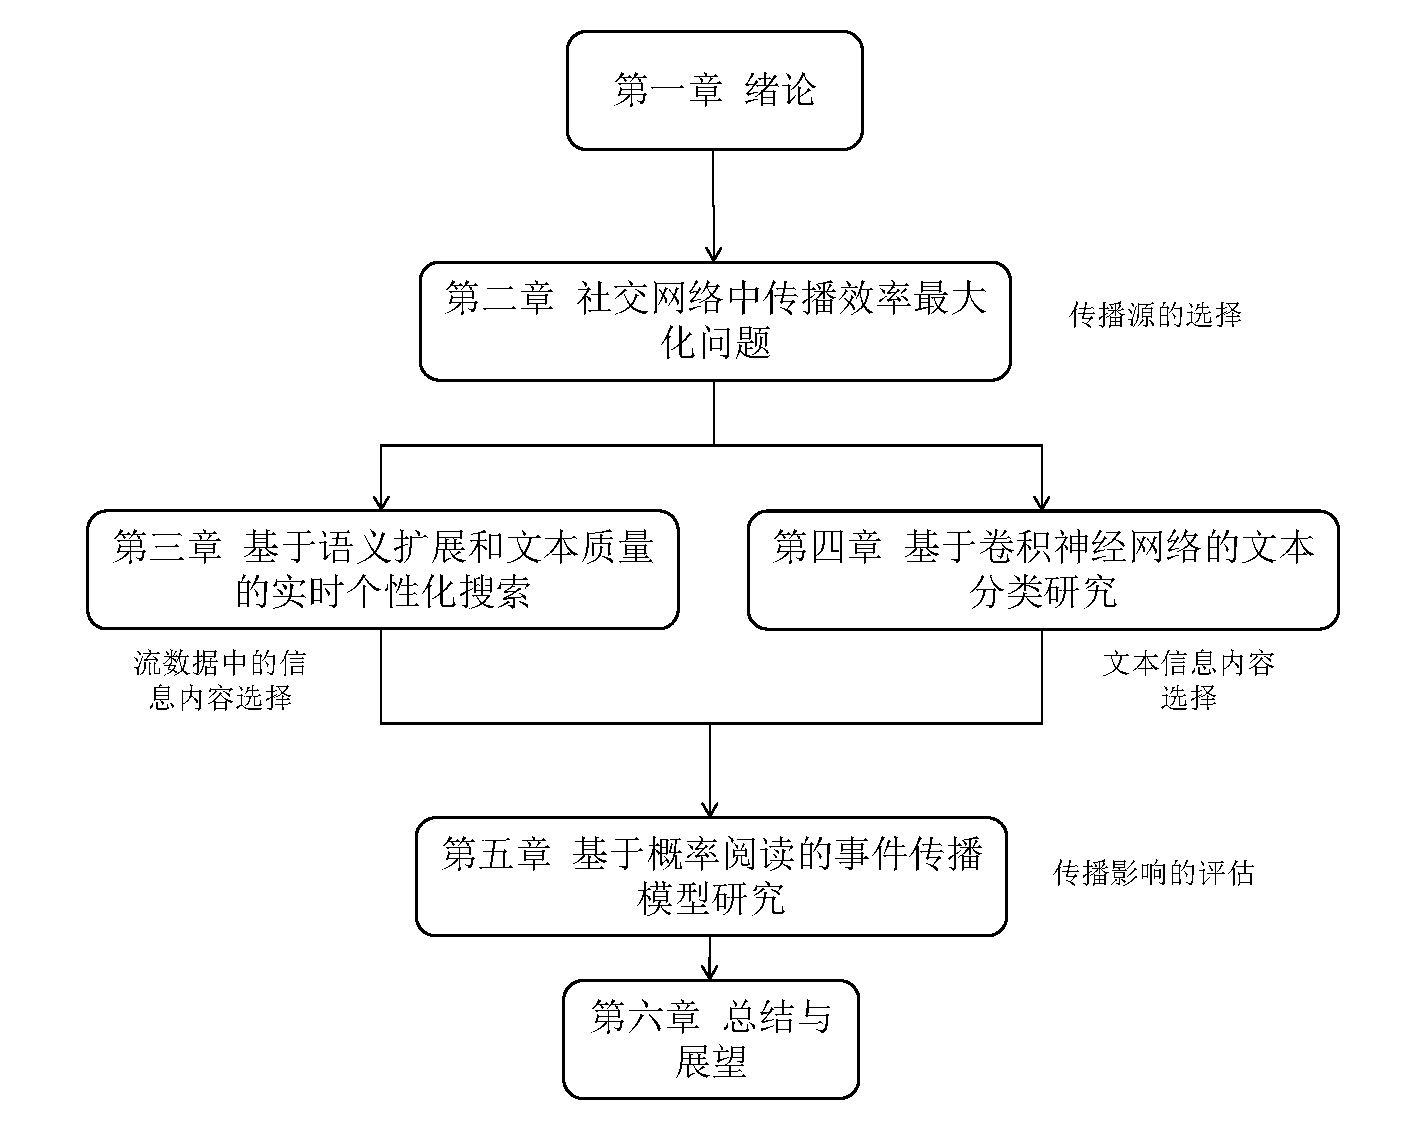
\includegraphics[width=0.8\textwidth]{paperStructure}
    \caption{论文组织结构图}
    \label{fig:paperStructure}
\end{figure}

第一章为绪论,阐述了本文的研究背景与与研究意义,同时对已有的相关研究工作进行了详细的总结,并且概括了本文的研究内容以及创新点。

第二、三、四、五章分别对社交网络信息传播的不同问题进行了研究。第二章研究在社交网络中如何选择传播源的问题,基于传统的影响力最大化问题,考虑传播时延,提出了传播效率最大化问题。第三、四章分别在不同的场景下研究如何选择传播内容的问题。第三章面向社交网络中的流数据,结合语义扩展以及质量模型提出了实时个性化搜索的框架。第四章面向社交网络中的文本数据,应用深度学习技术,提出了一种基于卷积神经网络的文本分类算法。第五章研究社交网络中信息传播的量化问题,以事件为粒度,结合多源信息网络融合、垃圾用户去重以及概率阅读模型,提出了一种新的传播模型用于衡量事件的传播范围。

第六章对本文的工作进行了总结,并对本领域的下一步研究进行了展望。